\part{Modelo a Escala}

Finalmente, se implementó un modelo a escala en el que se buscó alcanzar la falla por licuefacción, calibrar el modelo de diferencias finitas y comparar los resultados obtenidos. El objetivo de esta sección es visualizar toda la teoría anteriormente expuesta, observando las líneas de flujo, el caudal de infiltración, entre otros.

\section{Teoria}

\subsection{Escalamiento}
El análisis dimensional se utiliza para estudiar cómo cambian las fuerzas y el flujo al escalar un sistema como una ataguía. Se utilizan grupos adimensionales como el número de Reynolds, Froude y Euler.

\subsubsection{Número de Froude}
El número de Froude es importante cuando hay una superficie libre en el agua. Se calcula como:

\begin{equation}
Fr = \frac{V}{\sqrt{g L}}
\end{equation}

Donde:
\begin{itemize}
    \item $V$ es la velocidad del flujo,
    \item $g$ es la aceleración de la gravedad,
    \item $L$ es la altura de la ataguía.
\end{itemize}

Mantener el número de Froude constante ayuda a asegurar que el flujo tenga un comportamiento similar en un modelo a escala.


\subsection{Similitud en el Escalamiento}
Para que un modelo a escala sea válido, se deben cumplir tres tipos de similitud:

\begin{itemize}
    \item \textbf{Similitud geométrica}: Las dimensiones del modelo deben ser proporcionales a las del prototipo real.
    \item \textbf{Similitud cinemática}: El patrón de movimiento del agua debe ser igual en el modelo y en el sistema real, lo que se asegura manteniendo constante el número de Froude.
    \item \textbf{Similitud dinámica}: Las fuerzas que actúan deben ser proporcionales, lo que se logra manteniendo constantes números como $Re$ y $Eu$.
\end{itemize}

\subsection{Teorema de Buckingham $\pi$}

El teorema de Buckingham $\pi$ es un metodo para el análisis dimensional. Nos permite simplificar un sistema físico reduciendo sus variables dimensionales a un conjunto menor de grupos adimensionales $\pi$. Si un sistema tiene $n$ variables dimensionales y $k$ dimensiones fundamentales (como longitud, masa, y tiempo), entonces el número de grupos adimensionales es $n - k$.

Para comenzar se debe encintrar una relación funcional entre las $n$ variables dimensionales:

\begin{equation}
f(x_1, x_2, \ldots, x_n) = 0
\end{equation}

Según el teorema, esta relación puede reescribirse en términos de $n - k$ grupos adimensionales:

\begin{equation}
\pi_1 = \phi(\pi_2, \pi_3, \ldots, \pi_{n-k})
\end{equation}

Cada grupo $\pi$ es una combinación de las variables dimensionales del sistema, ajustadas para que el resultado sea adimensional. Los grupos $\pi$ tienen la forma general:

\begin{equation}
\pi_1 = x_1^{a_1} x_2^{a_2} \ldots x_n^{a_n}
\end{equation}

Los exponentes $a_1$, $a_2$, \ldots, $a_n$ se seleccionan de manera que las dimensiones de las variables se cancelen, haciendo que $\pi_1$ sea adimensional. El teorema asegura que cualquier relación física entre las variables dimensionales puede expresarse mediante estos grupos $\pi$, lo que facilita la simplificación y escalamiento de problemas físicos.

\subsection{Permeabilidad Muestra de Suelo}

Se define como permeabilidad aquella caracteristica del suelo que permite el paso del agua a travez de el \textbf{\cite{permeabilidad_suelos}}. Su unidades de medida son en Distancia/Tiemo donde existen diversas formas de estimar este coeficiente. En el caso de este proyecto, se midio un caudal con un gradiente hidraulico variable:

\begin{equation}
    k = \frac{a \cdot L}{A \cdot \Delta t} \cdot In(\frac{h1}{h2})
\end{equation}

Donde L corresponde a la altura de suelo, A el area transversal de suelo, $\Delta t$ el tiempo transcurrido, h1 y h2 las alturas de agua en el recipiente y a el ancho de la columna de agua.

\section{Resultados}

\subsection{Cálculo de Permeabilidad de la Muestra}

Para calcular la permeabilidad de la muestra se midio el tamiz que retuviera toda particula de suelo, de esta manera se puso un cono invertido sobre la malla, se agrego la muestra de suelo y se midio el tiempo que demoraba en pasar el agua. 

\begin{figure}[H]
    \centering
    \begin{minipage}{0.4\textwidth}
        \centering
        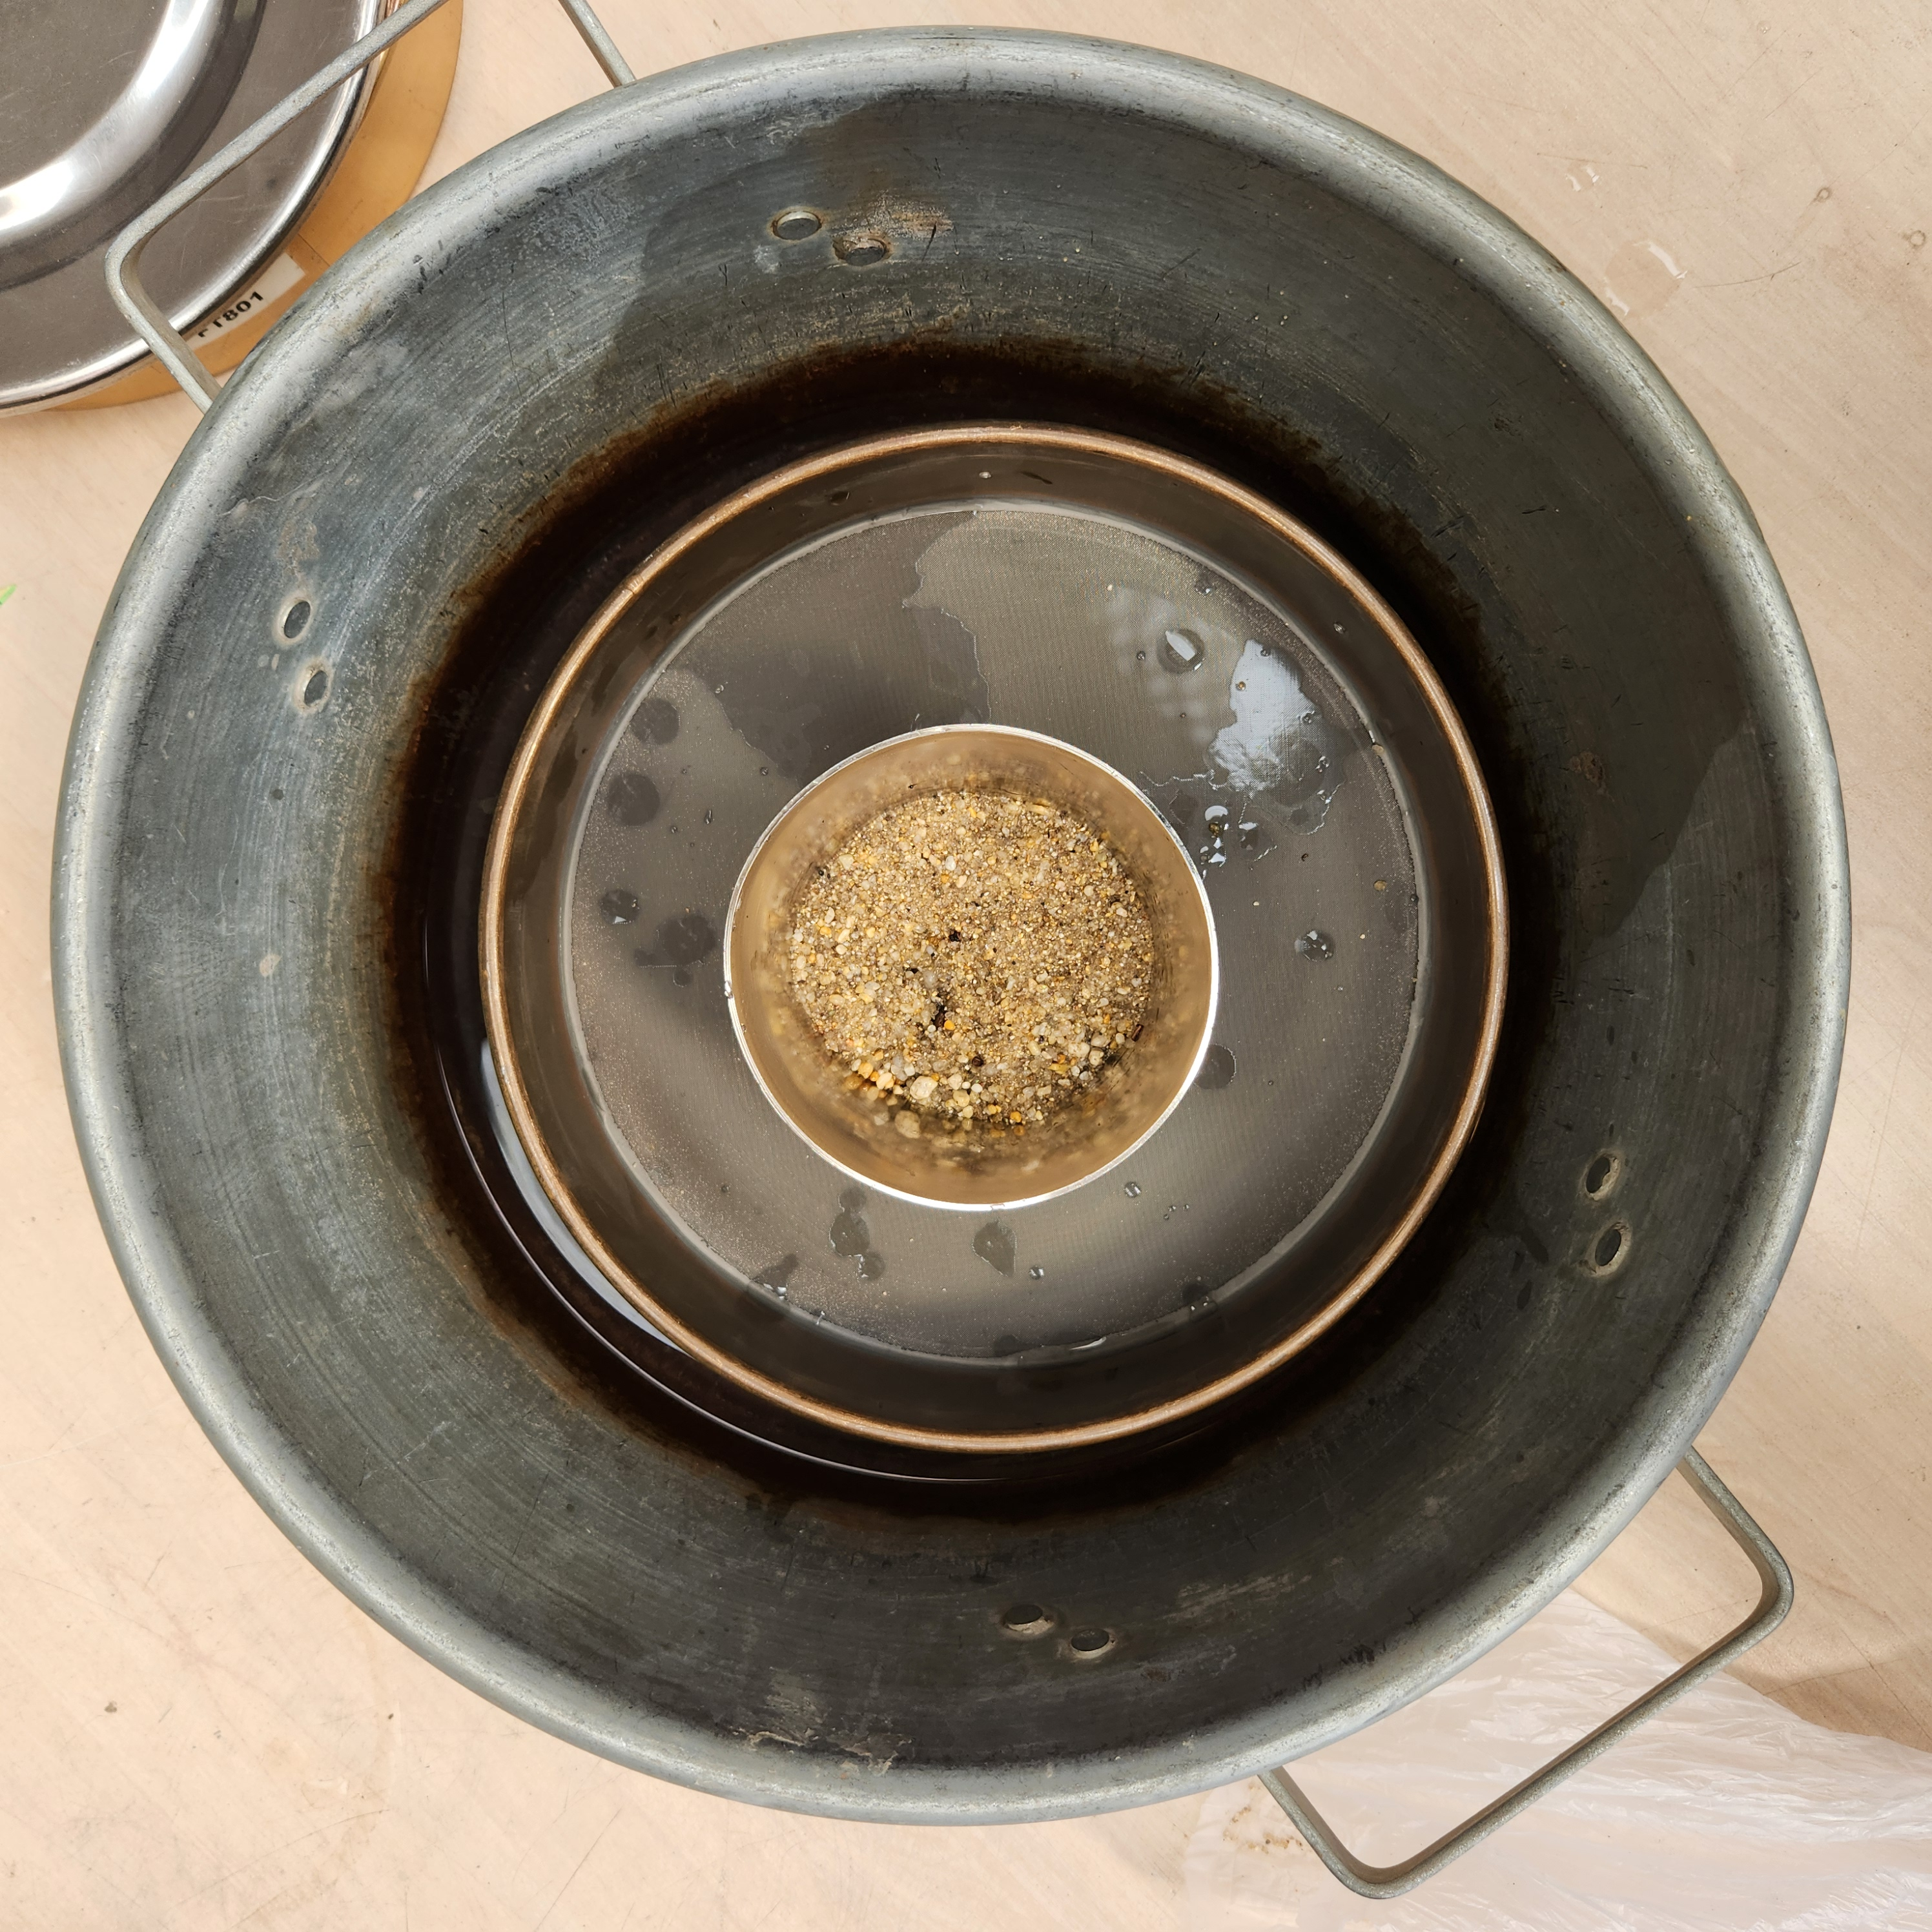
\includegraphics[angle=-90, width=\textwidth]{FOTOS/cono_1.jpg}
        \caption{Set Up Vista Superior}
    \end{minipage}
    \begin{minipage}{0.4\textwidth}
        \centering
        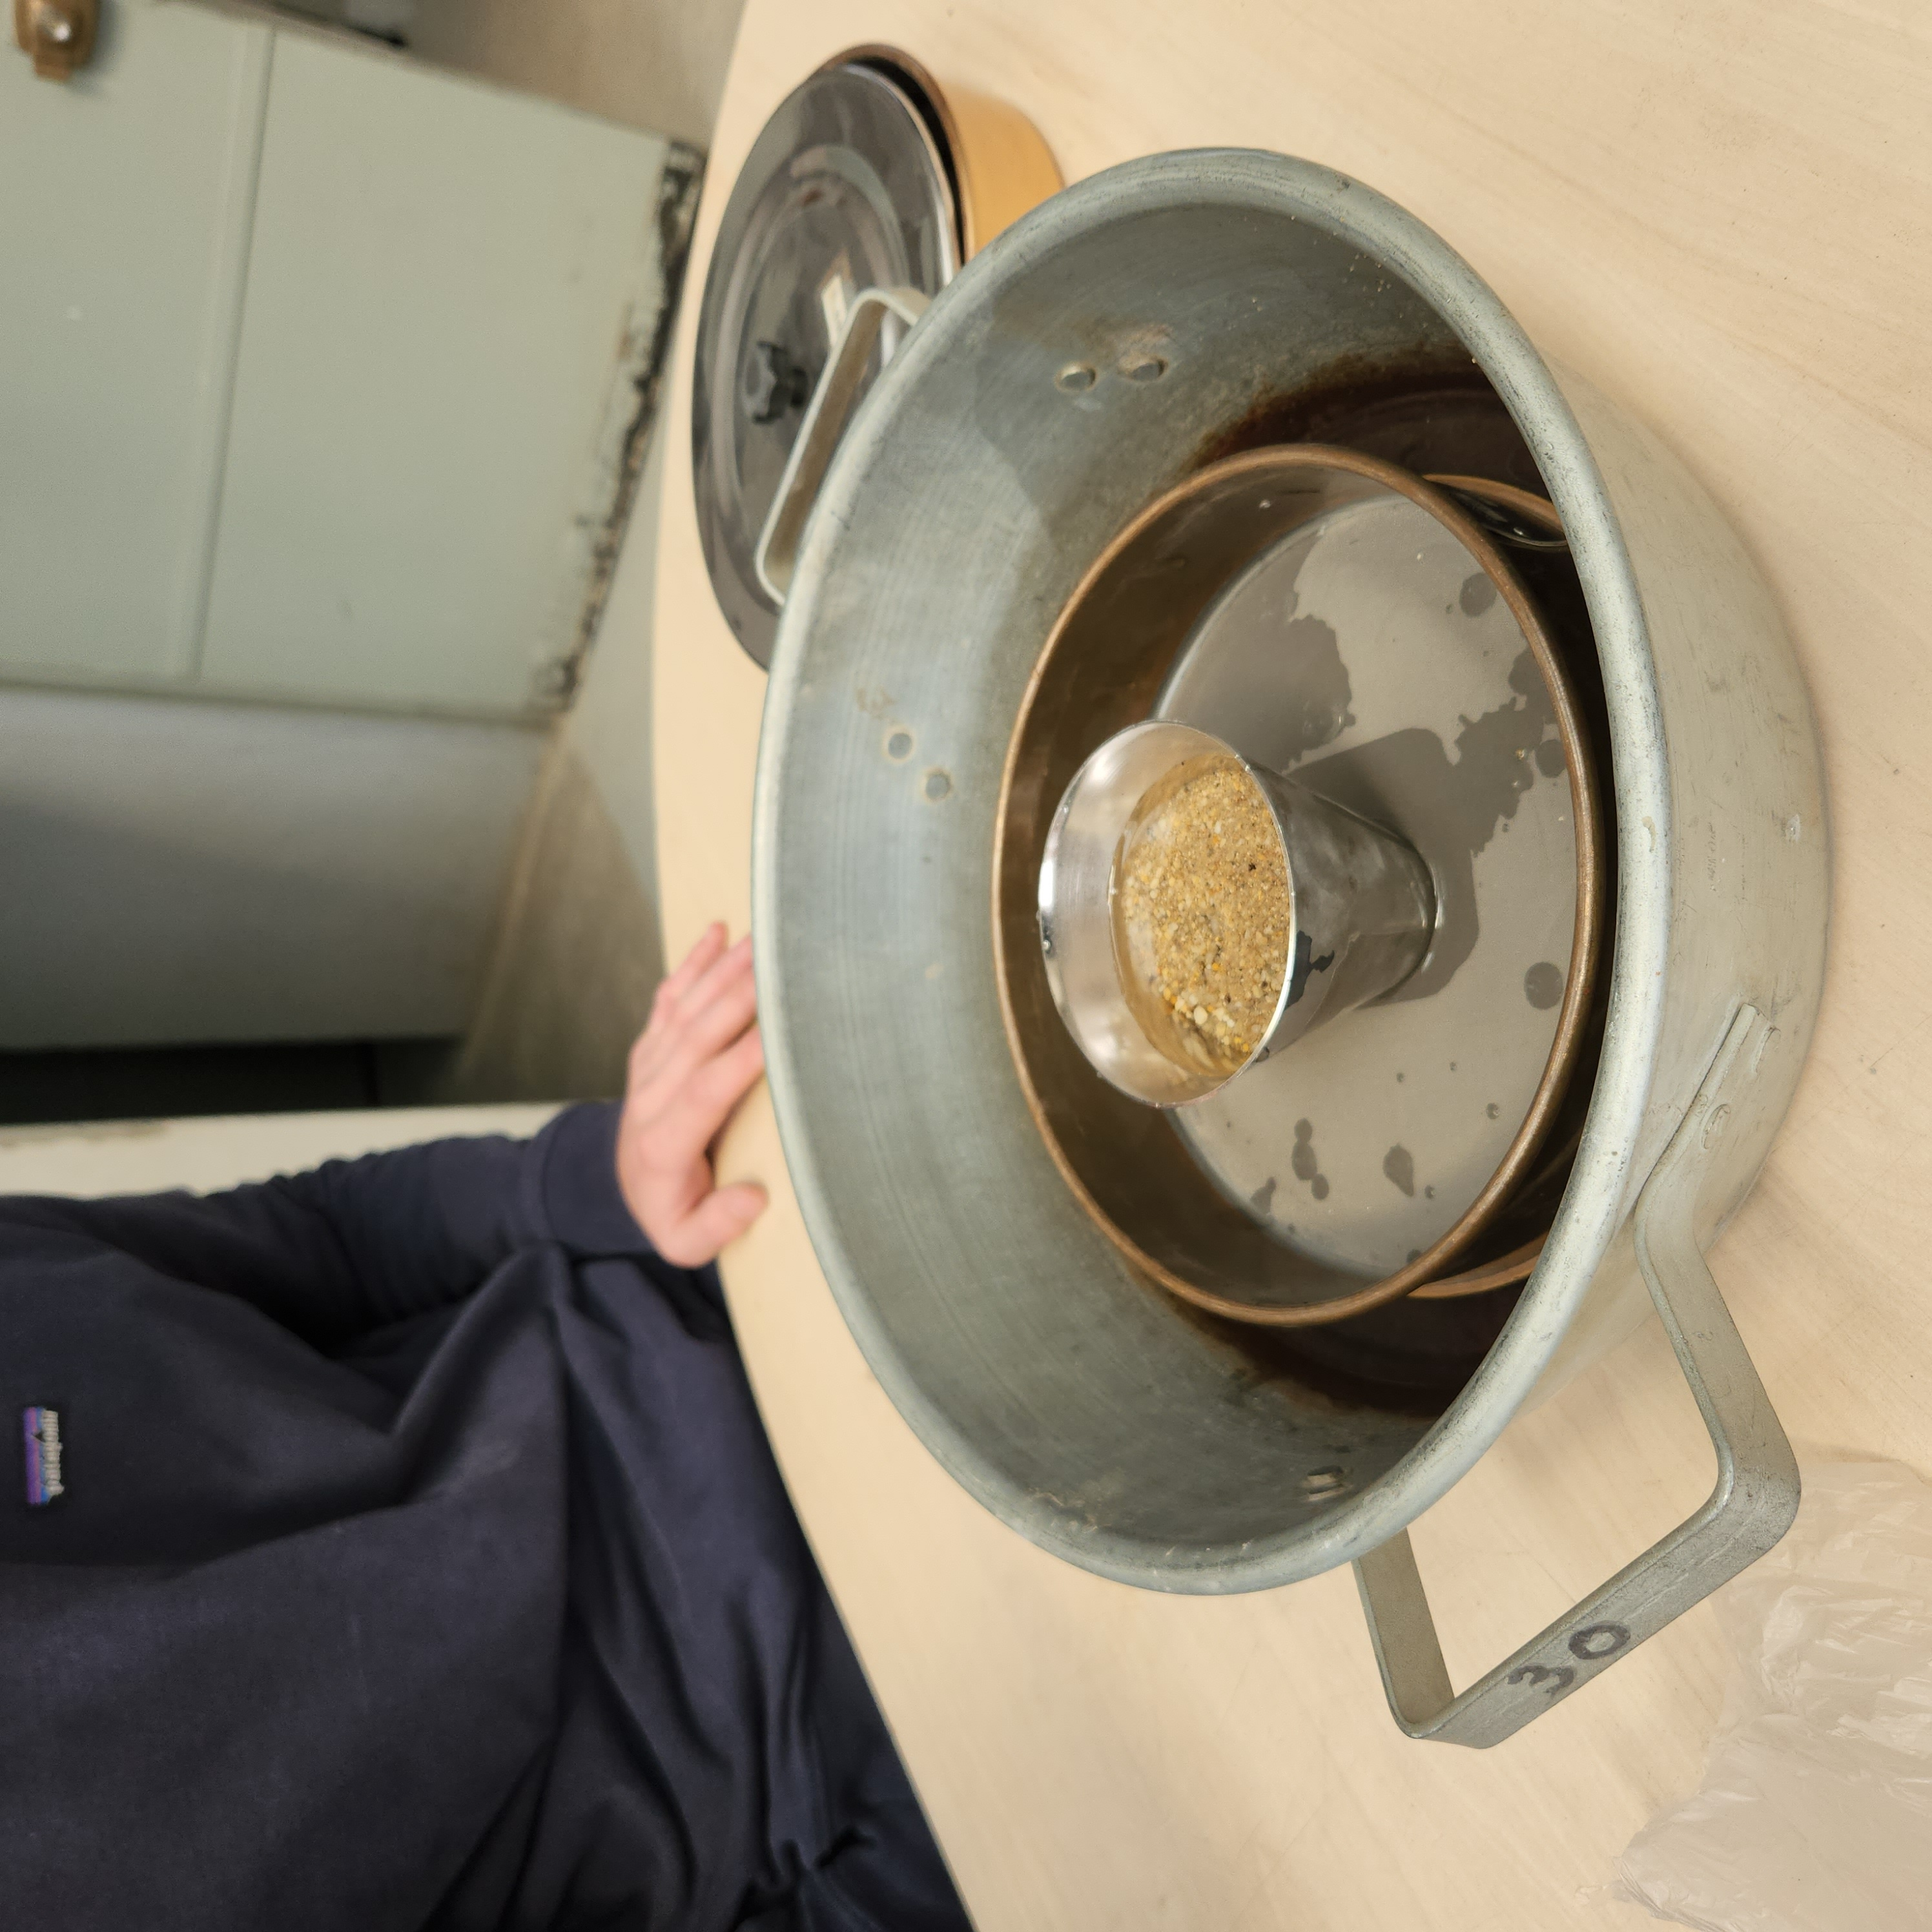
\includegraphics[angle=-90, width=\textwidth]{FOTOS/cono_2.jpg}
        \caption{Set Up Vista Lateral}
    \end{minipage}
\end{figure}

La toma de datos se realizo de la siguiente manera (ver en Adobe Acrobat):

\begin{center}
    \includemedia[
        width=0.5\textwidth, % Relación de aspecto 9:16 (altura mayor que el ancho)
        height=0.5\textwidth,
        activate=onclick,
        addresource=VIDEOS/permeabilidad.mp4,
        flashvars={
            source=VIDEOS/permeabilidad.mp4
        }
    ]{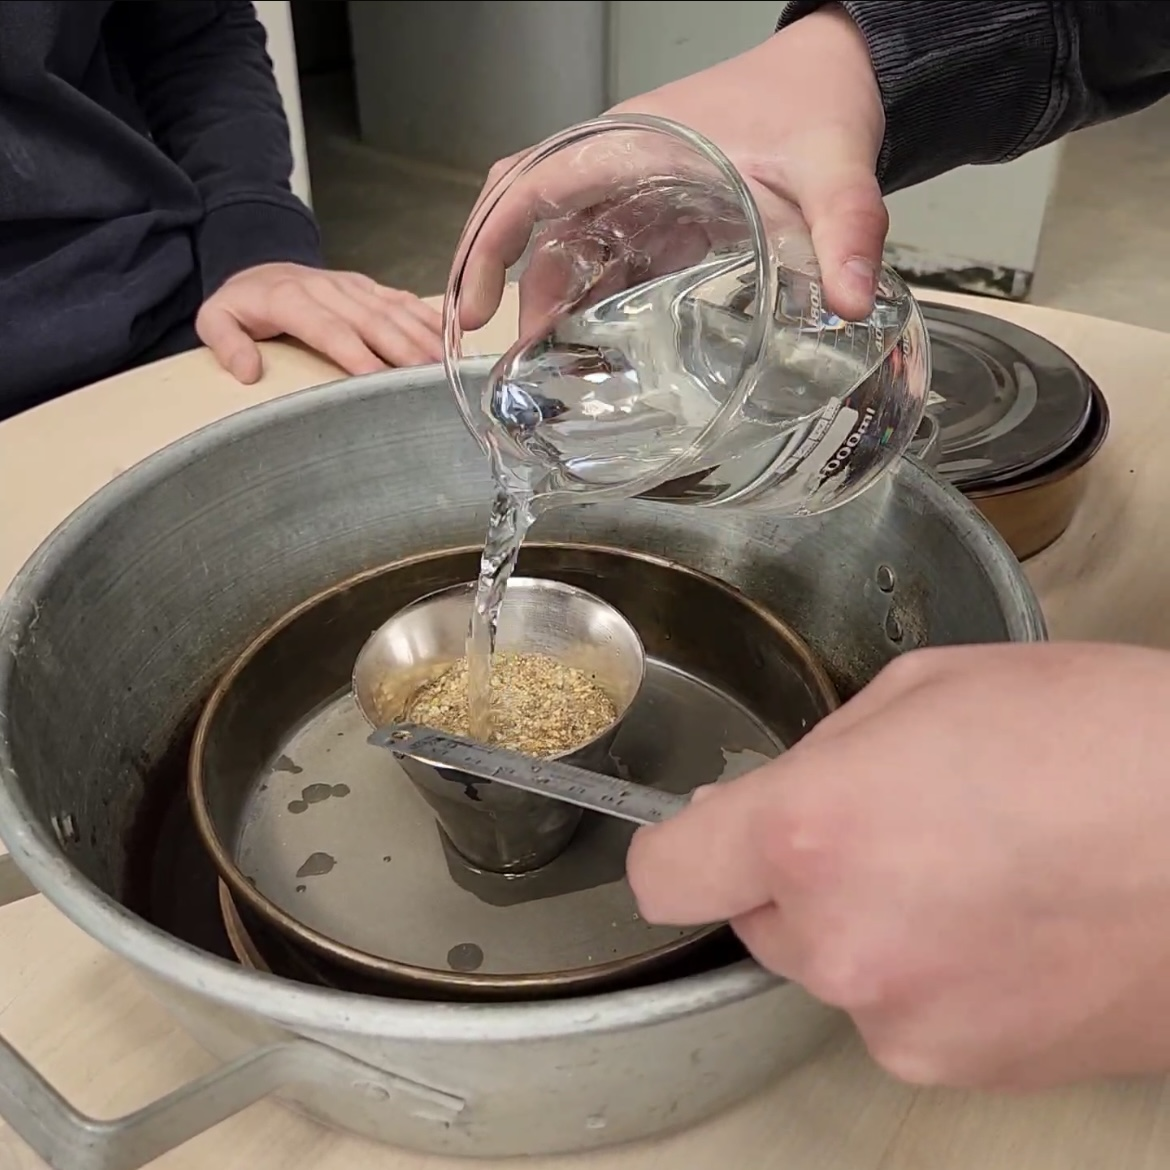
\includegraphics[width=\textwidth]{VIDEOS/miniatura_permeabilidad.jpg}}{VPlayer.swf}
\end{center}



Los datos obtenidos son los siguientes:


\subsection{Licuefaccion}

A continuación, se presenta un video (ver en Adobe Acrobat) de la falla observada por licuefacción en la maqueta a escala.

\begin{center}
    \includemedia[
        width=0.5625\textwidth, % Relación de aspecto 9:16 (altura mayor que el ancho)
        height=\textwidth,
        activate=onclick,
        addresource=VIDEOS/licuefaccion.mp4,
        flashvars={
            source=VIDEOS/licuefaccion.mp4
        }
    ]{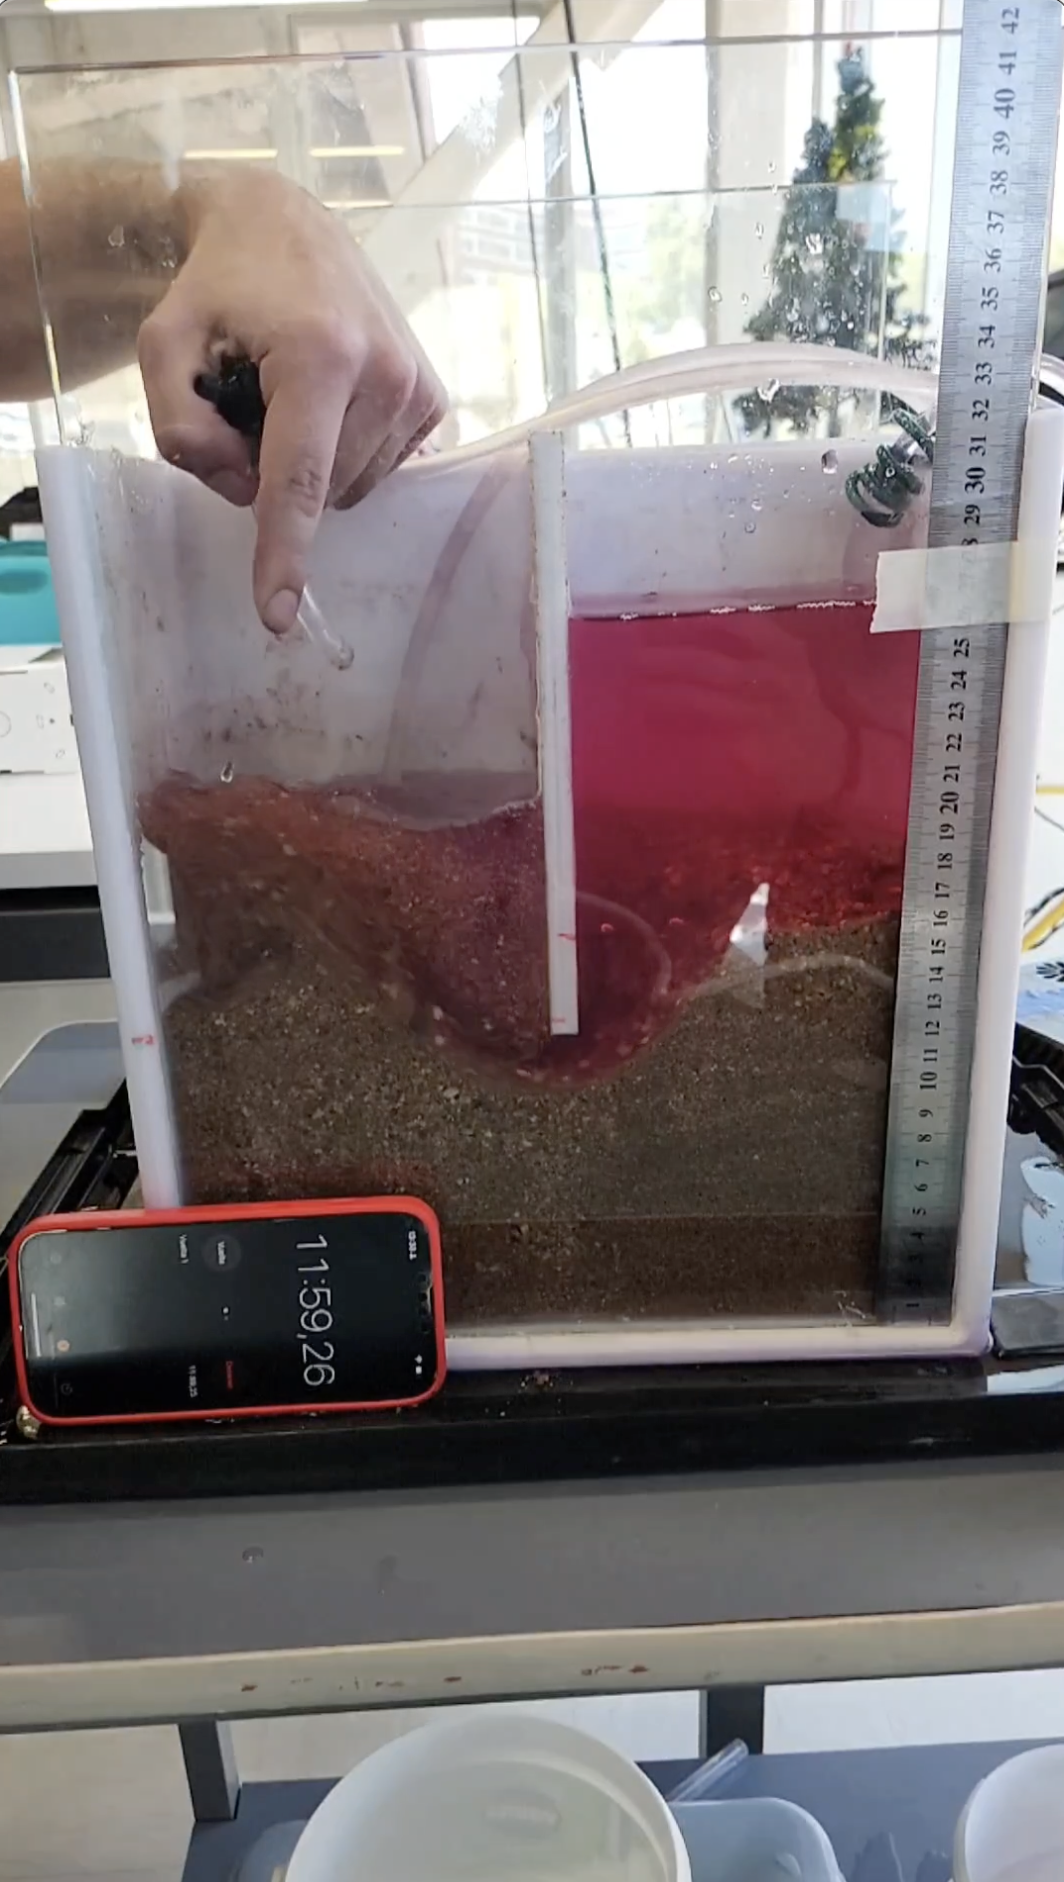
\includegraphics[width=\textwidth]{VIDEOS/miniatura_licuefaccion.png}}{VPlayer.swf}
\end{center}

Las medidas registradas son las siguientes:

\begin{table}[H]
    \centering
    \begin{tabular}{|c|c|c|c|c|c|c|c|}
    \hline
    Caso & $a_1$ & $b_1$ & $c_1$ & $a_2$ & $b_2$ & $c_2$ & $d$ \\ \hline
    Licuefacción & 0.0 & 14.5 & 15.5 & 15 & 2.5 & 12.5 & 0.5 \\ \hline
    \end{tabular}
    \caption{Medidas para la Licuefacción [cm]}
    \label{tab:medidas1}
\end{table}

Posteriormente, se realizó un mapa de calor correspondiente a la presión de poros durante la licuefacción:

\begin{figure}[H]
    \centering
    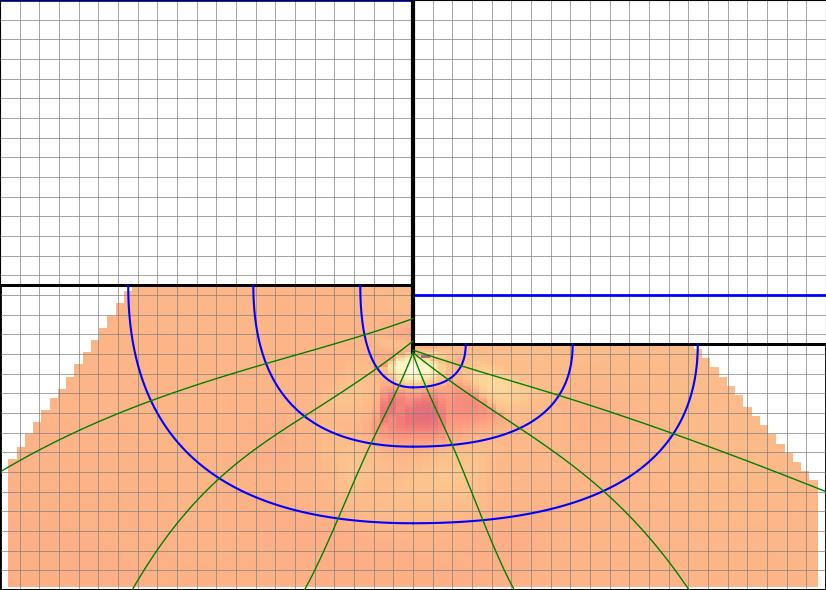
\includegraphics[width=0.5\textwidth]{GRAFICOS/caso_licuefaccion_presion_poros.jpg}
    \caption{Mapa de Calor de la Licuefacción}
    \label{fig:maqueta_licuefaccion}
\end{figure}

Es interesante notar cómo se produce un gran aumento de presión bajo la ataguía, lo cual se observa en el video, ya que ese es el punto esperado de falla.

Además, se calculó el mismo caso utilizando diferencias finitas:

\begin{figure}[H]
    \centering
    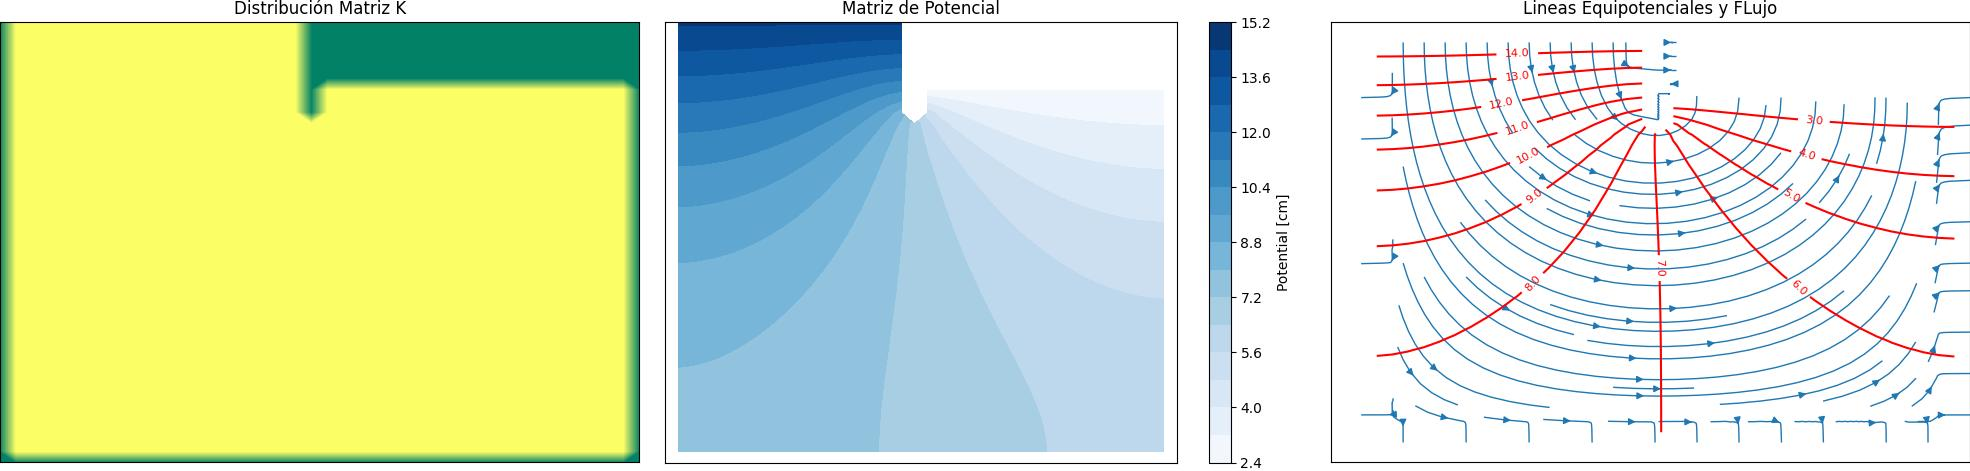
\includegraphics[width=1\textwidth]{GRAFICOS/laplace_caso_licuefaccion_escala_cm.jpg}
    \caption{Simulación con Diferencias Finitas del Caso de Licuefacción}
    \label{fig:maqueta_licuefaccion_diferencias_finitas}
\end{figure}

\subsection{Aplicación de Diferencias Finitas}

Se determina un caudal de 0.008972885614821659 cm/s

\subsection{Caudal escalado}

Mediante la confirmacion del teorema de Buckingham $\pi$ se obtiene que el caudal del modelo es:

\begin{equation}
    Q_{modelo} = Q_{prototopo} \cdot 1.1025 \cdot 10^{-4}
\end{equation}
